\subsection{Object Oriented Multi-Task Learning from Demonstration}
\label{sec:obj_oriented_multi_task_lfd}
As discussed in Section \ref{sec:baseline_definition}, the system is capable of generating valid trajectories but struggles to select the correct object. To test the hypothesis that enhancing the control module with low-level information, such as the target object's position, would simplify the control task and lead to improved performance, we trained a model similar to the one proposed in \cite{mandi2022towards_more_generalizable_one_shot}, but giving in input to the control module also the information about the target-object position, rapresented by the bounding box coordinates.
Consequently the novel system can be defined as a Conditioned-Policy $\pi^{L}_{\theta}(a_{t} | s_{t}, c_{m_{i}}, bb_{t}^{target})$ that generates the current action $a_{t}$ based on 3 inputs: \begin{enumerate*}[label=(\arabic*)]
    \item The current agent observation $s_{t} \in \mathbb{R}^{H \times W \times 3}$;
    \item The task command $c_{m_{i}} \in \mathbb{R}^{4 \times H \times W \times 3}$;
    \item The target-object bounding box $bb_{t}^{target} \in \mathbb{N}^{4}$.
\end{enumerate*}
\newline Table \ref{table:performance_with_bounding_box} provides a clear comparison between the outcomes achieved using the baseline approach and those achieved with our proposed method. We specifically applied two different variations for the analysis:
\begin{enumerate*}[label=(\arabic*)]
    \item The control module receives in input the Ground Truth (GT) bounding box;
    \item The control module receives in input the bounding box predicted with the module designed in Section \ref{sec:cond_target_obj_detector}.
\end{enumerate*}
\newline Table \ref{table:performance_with_bounding_box} reports the results obtained by adding the low-level bounding-box information to the control module.
\begin{table}[htb]
    \centering
    \fontsize{11pt}{11pt}
    \selectfont
    \caption{Performance comparison on pick-place and nut-assembly tasks, adding the information about the target object position}
    \label{table:performance_with_bounding_box}
    \resizebox{\linewidth}{!}{%
        \begin{tabular}{>{\centering\hspace{0pt}}m{0.192\linewidth}>{\centering\hspace{0pt}}m{0.35\linewidth}>{\centering\hspace{0pt}}m{0.142\linewidth}>{\centering\hspace{0pt}}m{0.115\linewidth}>{\centering\arraybackslash\hspace{0pt}}m{0.131\linewidth}}
            \hline
            \textbf{Task}                             & \textbf{Setup}             & \begin{tabular}[c]{@{}c@{}}\textbf{Reaching} \\\textbf{Rate }\\{[}\%]\end{tabular} & \begin{tabular}[c]{@{}c@{}}\textbf{Picking}\\\textbf{Rate }\\{[}\%]\end{tabular} & \begin{tabular}[c]{@{}c@{}}\textbf{Success}\\\textbf{Rate}\\{[}\%]\end{tabular} \\
            \hline
            \multirow{3}{*}{\Centering{}Pick-Place}   & Baseline                   & 66.8                                                                                                     & 64.3                                                                                                   & 58.7                                                                                                  \\
                                                      & Baseline with GT bb        & 100                                                                                                      & 96.5                                                                                                   & 76.8                                                                                                  \\
                                                      & Baseline with predicted bb & \textbf{97.5}                                                                                            & \textbf{92.5}                                                                                          & \textbf{78.1}                                                                                         \\
            \hline
            \multirow{3}{*}{\Centering{}Nut-Assembly} & Baseline                   & 40.0                                                                                                     & 38.8                                                                                                   & 36.6                                                                                                  \\
                                                      & Baseline with GT bb        & 100.0                                                                                                    & 98.8                                                                                                   & 60.0                                                                                                  \\
                                                      & Baseline with predicted bb & 3\textbf{8.8}                                                                                            & \textbf{38.8}                                                                                          & \textbf{26.6}                                                                                         \\
            \hline
        \end{tabular}
    }
\end{table}
From these results we can draw the following preliminary conclusions: \begin{enumerate*}[label=(\arabic*)]
    \item Incorporating bounding-box information proves to be beneficial for system performance. When the control module is provided with ground-truth data as input, it results in a consistent ability of the system to reach the target object and effectively accomplish the task. This enhancement is reflected in improved success rates for both the pick-place and nut-assembly tasks;
    \item While the introduction of the Conditioned-Target Object Detector module shows promising aspects, notably the substantial 19.4\% increase in success rate for the pick-place task, it also brings to light limitations tied to what is termed "error propagation". In other words, errors originating from an upstream module can influence subsequent modules in the system. This limitation becomes evident in the nut-assembly task, where there is a notable decline in performance. In this scenario, the prediction module encounters difficulties in accurately identifying the correct object, particularly during the initial frame. As a consequence, the robot ends up choosing the wrong object, as reported in Table \ref{table:baseline_with_bb_na} and illustrated in Figure \ref{fig:nut_assembly_error}. It's important to emphasize that we did not observe this phenomenon in Section \ref{sec:cond_target_obj_detector}. In that case, the module initially generated a false-positive prediction in the first frame. However, once the robot made its first movement toward the correct object, the subsequent predictions were accurate. This observation suggests the potential existence of a correlation between the position of the robot's arm and the predicted bounding box.
\end{enumerate*}
\begin{table}[bth!]
    \caption{Relevant error cases in pick-place task (\ref{table:baseline_with_bb_pp}) and nut-assembly task (\ref{table:baseline_with_bb_na})}
    \label{table:baseline_with_bb_error_cases}
    \begin{subtable}[h]{0.45\textwidth}
        \centering
        \fontsize{9pt}{9pt}
        \selectfont
        \caption{Relevant error cases in pick-place task}
        \label{table:baseline_with_bb_pp}
        \resizebox{\linewidth}{!}{%
            \begin{tblr}{
                cells = {c},
                hlines,
                hline{1,5} = {-}{0.08em},
                    }
                \textbf{Error case} & \textbf{\#Occurrences} \\
                Wrong bin           & 17                     \\
                Fail to pick        & 9                      \\
                Other               & 8
            \end{tblr}
        }
    \end{subtable}
    \hfill
    \begin{subtable}[h]{0.45\textwidth}
        \centering
        \fontsize{9pt}{9pt}
        \selectfont
        \caption{Relevant error cases in nut-assembly task}
        \label{table:baseline_with_bb_na}
        \resizebox{\linewidth}{!}{%
            \begin{tblr}{
                cells = {c},
                hlines,
                hline{1,5} = {-}{0.08em},
                    }
                \textbf{Error case} & \textbf{\#Occurrences} \\
                -                   & -                      \\
                -                   & -                      \\
                -                   & -
            \end{tblr}
        }
    \end{subtable}

\end{table}
\begin{figure}[bth!]
    \centering
    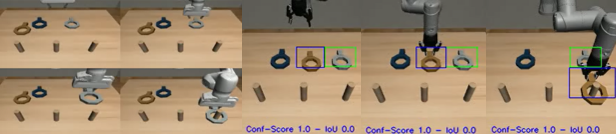
\includegraphics[width=0.9\textwidth]{Figures/images/nut_assembly_error/nut_assembly_error.png}
    \caption{Example of error for nut-assembly task. The robot picks the wrong object due to a false positive generated by the bounding-box predictor}
    \label{fig:nut_assembly_error}
\end{figure}


In conclusion, the proposed approach has initiated the validation of the hypothesis that dividing the Decision-Making Process into two stages, with explicit handling of a task associated with the Command-Analysis stage, could potentially yield a more robust system. However, there are several areas where improvements are needed, particularly concerning the Conditioned-Target Object Detector. Enhancements should focus on improving the initial frame predictions to minimize object confusion and the potential correlation with the position of the robot's arm. These improvements can be achieved through the application of appropriate data augmentation techniques, such as introducing bounding boxes that do not encompass any objects and categorizing them as ``no-target", or by adding random patches within the robot's arm region. Furthermore, following this validation in a simulated environment, our next step is to extend the modules to a real-world controlled setting, leveraging the framework described and detailed in Section \ref{sec:dataset_description}.